\documentclass{article}
\usepackage{amsmath, amssymb, cite, algorithmic, url, braket}
\usepackage{graphicx}
\usepackage{pythonhighlight}
\usepackage[margin=1.5cm]{geometry}
\usepackage[title]{appendix}
\usepackage{listings}
\usepackage{booktabs}

\graphicspath{{../pic/}}
\lstset{
language=[ANSI]{C},
showtabs=true,
tab=,
tabsize=2,
basicstyle=\ttfamily\footnotesize,%\setstretch{.5},
stringstyle=\color{stringcolour},
showstringspaces=false,
alsoletter={1234567890},
otherkeywords={\%, \}, \{, \&, \|},
keywordstyle=\color{keywordcolour}\bfseries,
upquote=true,
morecomment=[s]{/*}{*/},
commentstyle=\color{commentcolour}\slshape,
literate=*%
{=}{{\literatecolour=}}{1}%
{-}{{\literatecolour-}}{1}%
{+}{{\literatecolour+}}{1}%
{*}{{\literatecolour*}}{1}%
{!}{{\literatecolour!}}{1}%
{[}{{\literatecolour[}}{1}%
{]}{{\literatecolour]}}{1}%
{<}{{\literatecolour<}}{1}%
{>}{{\literatecolour>}}{1}%
% {>>>}{\pythonprompt}{3}%
,%
frame=trbl,
rulecolor=\color{black!40},
backgroundcolor=\color{white},
breakindent=.5\textwidth,frame=single,breaklines=true
}

\begin{document}
\title{DSP Homework 06}
\author{Xu, Minhuan}
\maketitle
\tableofcontents
\begin{abstract}
    \subsubsection*{Videos}
        To sum up the videos we watched this week.
    \subsubsection*{Sampling Method developed with Fourier Series}
        According to Fourier series, the sampling method using $\delta(t)$ will involve infinity energy which is not realizable. So, I try to develop a new method.
\end{abstract}

\section{Summary and Thoughts}

\subsection{Bluetooth}
In this video, we know about the technique about Bluetooth, I found something special about the Bluetooth as below.

\subsubsection*{Points Worth Noting}
\begin{enumerate}
    \item Working on $123~\mathrm{mm}$ wave length EM wave
    \item Using $120.7~\mathrm{mm}$ represent 1, $124.9 ~ \mathrm{mm}$ represent 0
    \item Sending a Million Bits per Second in the format of {Packets} \label{enum:packets}
    \item Having $79$ Communication Channel and {shifting} among them continuously \label{enum:shifting}
\end{enumerate}

In these points, I want to write more about \ref{enum:packets}. and \ref{enum:shifting}.

\subsubsection*{Packets}
The packets are a set of lots of $'0'$ and $'1'$. 

First $72$ bits are called {Access Code}, which are used to synchronize smartphone and earbuds to make sure that it's your specific earbuds that is that received the message. 

Next $54$ bits are called {Header}. These data are used to decide how much data should be transfer next.

Last $136 \sim 8186$ bits are called {Payload}. There will be control signals like pause and play or music data in this part. So, this part can be long and short which is decided by the {Header} part.

\subsubsection*{Frequency Hopping Spread Spectrum}
My understanding is there is a list of the number of $79$ Communication Channels. The phone and the earbuds should use different channel once a packet is transferred. So, the list decides in which order the Communication Channels are used.

\subsubsection*{Time slots}
The Bluetooth protocol states that a packet should be transferred in $625~ \mathrm{\mu s}$, and the earbuds and the phone alternately use a time slot for data transmission.


\subsection{Learning to Learn}
This is a lecture about why we should keep learning and how we can learn better.
\subsubsection*{Life-long Learning}
The lecturer made a list of famous rich people, and try to make audience find out the similarity among them. And it turns out that the most precious ability is life-long learning. So, as the lecturer said, our learning ability decides our earning capacity. I don't quite know whether this is right, but keeping on learning new things on a regular basis won't be bad.

\subsubsection*{More OUTPUT rather than INPUT}
Saying goes that, knowledge, use it or lose it. Here's some suggestions about learning from the lecturer.

\begin{enumerate}
    \item Focus on what we learn, in other words, do single-tasking, or we will kill our motivation
    \item Reflect what we learn, in other words, don't read and wait for forgetting
    \item To implement is far more better than just remembering
    \item Share our knowledge with others, which is good for ourselves
\end{enumerate}

\subsection{Further Thoughts}
In the Frequency Hopping Spread Spectrum technology, I don't fully understand how to keep the sender and the receiver knowing which channel to use next. So, I searching for how it works and I find that the Bluetooth protocol states that there must be a PIN code if the two devices want to pair. Then, the number of channels will be generated by pseudo-random code which is decided by the PIN code, so if other devices don't know the PIN  code, it's impossible to hijack.


\section{My Sampling Method}

\subsection{Restatement}
Use the Fourier series to develop a sampling method and compare it with the Shannon/Nyquist sampling method through
examples.
\subsection{Derivation}
In class, we are considering the energy of the Fourier transform of the $s(t)$, we have
\begin{equation}
s(t) = \sum_{n = -\infty}^{\infty} c_n \, e^{j2 \pi n fT}
\end{equation}
and we have
\begin{equation*}
\begin{aligned}
E &= \int_{-\frac{T}{2}}^{\frac{T}{2}} \, s(t) \cdot s^*(t) \, \mathrm{d}t \\ 
% &= \int_{-\frac{T}{2}}^{\frac{T}{2}} \, \sum_{n = -\infty}^{\infty} c_n \, e^{-j2 \pi n fT} \cdot \sum_{m = -\infty}^{\infty} c_m e^{j2 \pi m fT} \, \mathrm{d}t \\ 
&= \int_{-\frac{T}{2}}^{\frac{T}{2}} \, \sum_{n = -\infty}^{\infty} c_m \cdot c_n ~ e^{j2 \pi (n - m) fT}  \, \mathrm{d}t \\ 
&= \sum_{n = -\infty}^{\infty} c_m \cdot c_n ~ \int_{-\frac{T}{2}}^{\frac{T}{2}} ~ e^{j2 \pi (n - m) fT}  \, \mathrm{d}t \\ 
\end{aligned}
\end{equation*}
and the integral of $e^{j2 \pi (n - m) fT}$ usually be $0$ except that $n - m$, so
$$
E =\sum_{n = -\infty}^{\infty} c_n^2 \cdot T
$$

I will try to prove that if $E < \infty$, we must ensure that $n \to \infty, c_n \to 0$, which means 
\begin{equation}
E < \infty \Rightarrow  n \to \infty, c_n \to 0
\label{eq:energyInfty}
\end{equation}

if that
$$
n  \to \infty, c_n \to C \, (C \neq 0)
$$
we can always find a big number $N$ which makes $c_n^2 > 0 \, (n > N) $, and we can easily find that
$$
\sum_{n = N}^{\infty} c_n^2 > (\infty - N) \cdot c^2_{n(min)} \to \infty
$$

So, $E\to \infty$ when $n  \to \infty, c_n \to C \, (C \neq 0)$.
Therefore, Equa.\ref{eq:energyInfty} is proved. Next, we need to find a energy-limited signals to do the sampling.
And we know that
\begin{equation*}
    c_n = \frac{1}{T} \int_{-\frac{T}{2}}^{\frac{T}{2}} s(t) \, e^{-j2\pi n f_s t} \, \mathrm{d}t
\end{equation*}

So, the same as I find out last week in my weekly report, we know that if we let the square impulse have the width of $2\tau$, we now have
\begin{equation}
    \begin{aligned} s(t) & = \sum_{n = -\infty}^{\infty} \mathrm{rect} (\frac{t - nT}{\tau}) \\
             & = \sum_{n =-\infty}^{\infty}F_n e^{j2 \pi n f_s t}  \\
             & = \sum_{n = -\infty}^{\infty}\left[ \frac{1}{T} \int_{-\frac T2}^{\frac T2}
              \mathrm{rect}(\frac{t}{\tau}) e^{-j2 \pi n f_s t} \mathrm{d}t \right] e^{j2 \pi n f_s t} \\
             & = \sum_{n = -\infty}^{\infty}\left[ f_s \int_{-\tau}^{\tau} e^{-j2 \pi n f_s t} \mathrm{d}t \right] e^{j2 \pi n f_s t}  \\
             & = \sum_{n = -\infty}^{\infty}2f_s\, \mathrm{sinc} \,( 2f_s n\tau)\, e^{j2 \pi n f_s t} \\
             \label{eq:samplingSquare}
    \end{aligned}
\end{equation}

Here, 
\begin{align*}
\begin{array}{lrl}
s(t) &=& \sum\limits_{n = -\infty}^{\infty} \mathrm{rect} (\frac{t - nT}{\tau}) \\ \\
c_n  &=& 2f_s\, \mathrm{sinc} \,( 2f_s n\tau)
\end{array}
\end{align*}  

% According to the document on the Internet\cite{sinc_sum}, I know that
% \begin{equation}
% \sum_{n = -\infty}^{\infty} \, sinc(nT) = \frac{\pi}{T}
% \end{equation}

Therefore
\begin{equation}
\begin{aligned}
E &= T \cdot \sum_{n = -\infty}^{\infty} c_n^2 \\ 
&= T \cdot \sum_{n = -\infty}^{\infty} sinc^2(2f_sn\tau)
\end{aligned}
\label{eq:EnergySeries}
\end{equation}

\newpage

In help of Wolfram Alpha \cite{sinc_convergence}, I know that when a is real, this series (Eq.~\ref{eq:EnergySeries}) converges. 
The result is shown in Fig.~\ref{fig:sinc_convergence}.

\begin{figure}[htbp]
    \centering
    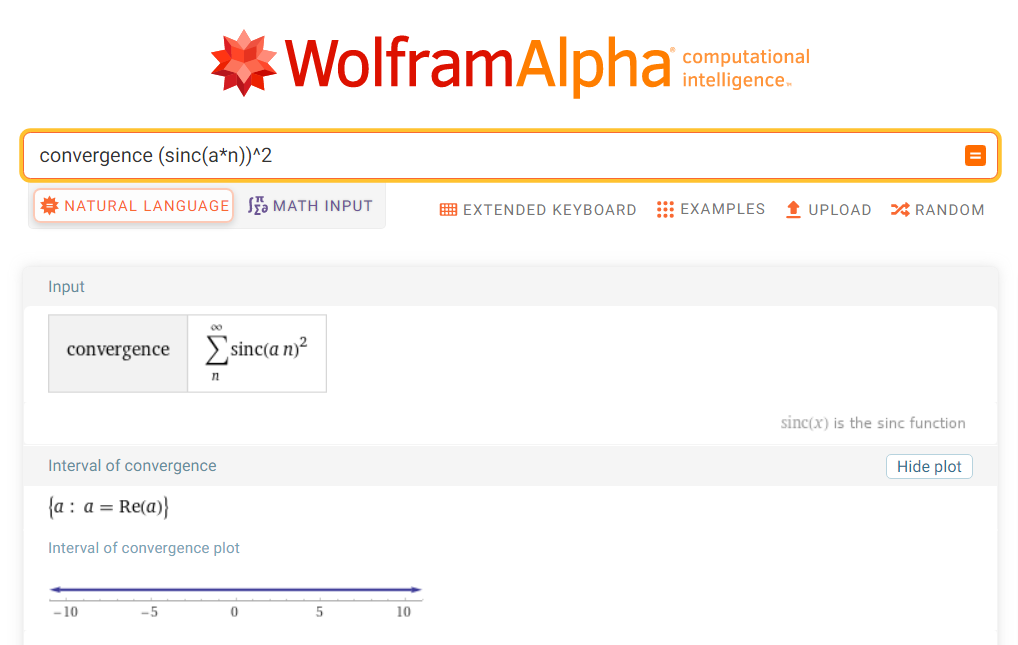
\includegraphics[keepaspectratio,width=250pt]{../pic/sinc_convergence.png}
    \caption{Convergence of $sinc^2(a\times n)$}
    \label{fig:sinc_convergence}
\end{figure}

% $$
% \sum_{n = -\infty}^{\infty} sinc^2(a\times n) < \infty
% $$

Therefore
\begin{equation*}
\sum_{n = -\infty}^{\infty} sinc^2(2f_sn\tau) < \infty
\end{equation*}

we can now say that the $s(t)$ mentioned in Equa.\ref{eq:samplingSquare} is energy-limited.

And back to Equa.\ref{eq:EnergySeries}, we can control the order of the sum to improve this equation because the $c_n$ decrease rapidly. Therefore
$$
E = T \cdot \sum_{n = -N}^{N} sinc^2(2f_sn\tau)
$$
So, let's use python to draw a picture to see more clearly, see Fig.~\ref{fig:sincAndLine}.

\begin{figure}[!h]
    \centering
    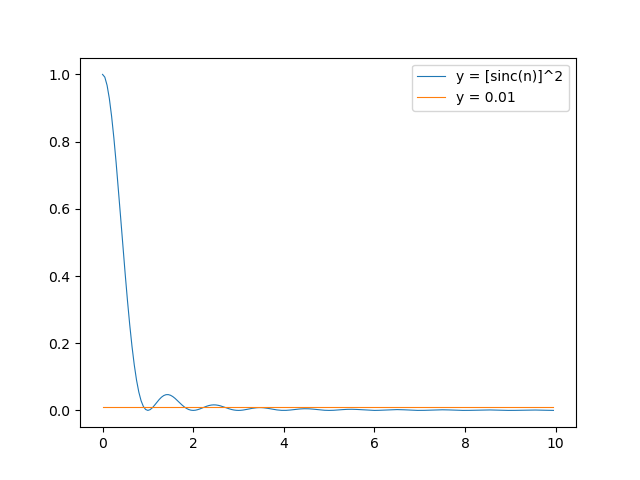
\includegraphics[width=3 in]{../pic/sincAndLine.png}
    \caption{Orders of Sinc Function}
    \label{fig:sincAndLine}
\end{figure}
It's easy to find that if we make $n$ in this picture less than $5$ or even $3$ , little energy will be lost. This means we can rewrite the Equa.~\ref{eq:EnergySeries} like
\begin{equation}
E = T \cdot \sum_{n = -N}^{N} sinc^2(2f_sn\tau) \qquad N = [\frac{5}{2f_s \tau}] + 1
\label{eq:improvedEnergy}
\end{equation}

If we look back on the $\delta(t)$ sampling, we have the energy $E$ of $s(t)$:
\begin{equation}
E = \sum_{n = -\infty}^{\infty} T \to \infty
\label{eq:impulseEnergy}
\end{equation}
This (using $\sum \delta(t)$ to sampling) is not realizable. And, we can say that not the square function, but all energy-limited signals may be good for sampling.

\section{Conclusion}
    \subsubsection*{Videos}
        After doing the summary of these videos, I further researched something about FHSS.
    \subsubsection*{Sampling Method developed with Fourier Series}
        With the help of Fourier Series, I proved that it is more realizable to sample other signals with energy-limited signals like square function.
\bibliographystyle{ieeetr}
\bibliography{../bib/database}

\begin{appendices}
\section{Code Listing}
\begin{python}
    import numpy as np
    from sympy import sinc
    from matplotlib import pyplot as plt

    n = np.arange(0.7, 5, 0.01)
    y = (np.sinc(n))**2
    line = [0.01 for x in n]

    fig = plt.figure()
    plt.plot(n, y, linewidth=0.8, label="y = [sinc(n)]^2")
    plt.plot(n, line, linewidth=0.8, label="y = 0.01")
    plt.legend()
    plt.show()
\end{python}

\end{appendices}

\end{document}